\section*{Exercício 7}
\label{ex:7}
\raggedbottom

Os dados utilizados na simulação tanto da planta quanto dos controladores estão nas tabelas \ref{tab:ex7planta} e \ref{tab:ex7controlador}. 

\begin{table}[H]
    \centering
    \begin{tabular}{|l|c|c|c|}
    \hline
    Descrição & Símbolo & Unidade & Valor \\ \hline
    Resistência do estator & R & $\Omega$ & 1 \\
    Indutância do estator & L & H & 0.5 \\
    Momento de inércia & J & kg $m^2$  & 0.01 \\
    Coeficiente de atrito viscoso & b & $Ns$ & 0.1 \\
    Fator transformação eletromagnética & K & NmA & 0.01 \\\hline
    \end{tabular}
    \caption{Parâmetros da planta}
    \label{tab:ex7planta}
\end{table}

\begin{table}[H]
    \centering
    \begin{tabular}{|l|c|c|c|}
    \hline
    Descrição & Símbolo & Unidade & Valor \\ \hline
    Ganho proporcional & $K_p$ & $N \frac{rad}{s}$ & 18 \\
    Constante de tempo integrativo & $T_i$ & s & 0.42 \\
    Constante de tempo derivativo & $T_d$ & s  & 0.05 \\
    Período de amostragem & $T_s$ & s & 0.01 \\\hline
    \end{tabular}
    \caption{Parâmetros dos controladores}
    \label{tab:ex7controlador}
\end{table}

A utilização da estratégia anti-windup juntamente ao controlador PID reduz o tempo que o controlador necessita para sair da área de saturação. Na imagem \ref{fig:PIDantiwindup} o controlador PID clássico integra o erro, como se observa pela curva acentuada e crescente. A curva respectiva ao  controlador com \emph{anti-windup} rapidamente volta ao regime de não-saturação.

Ao compararmos controladores PID, ambos com estratégia anti-windup, sem e com filtro passa-baixas na ação derivativa na imagem \ref{fig:PIDfiltro}, não é possível observarmos uma diminuição na sensibilidade ao ruido de leitura, esperado pela sua natureza. Uma melhor abordagem é a implementação de um filtro analógico na saída do sensor de coleta dos dados a fim de evitar o efeito de \emph{aliasing} do sinal adquirido.

O aluno escolheu duas estratégias de controle PID anti-windup com filtro apresentadas na apostila da disciplina. A primeira não acresce a ação integral durante o período de saturação e a segunda, além da estratégia do anterior, mitiga o sinal de controle por meio de um fator proporcional à diferença de ação de controle antes e depois da saturação. Ambas apresentaram qualitativamente o mesmo desempenho, como se observa na imagem \ref{fig:PIDantiwindup12}.

Por fim, como análise final, o torque fornecido como perturbação no eixo do motor afeta de forma semelhante a velocidade durante seu período de atuação. Nos casos em análise, o motor não alcança a velocidade estacionária estabelecida. Entretanto, a velocidade angular converge para o valor de referência na ausência de distúrbio.

\begin{figure}[H]
    \center
    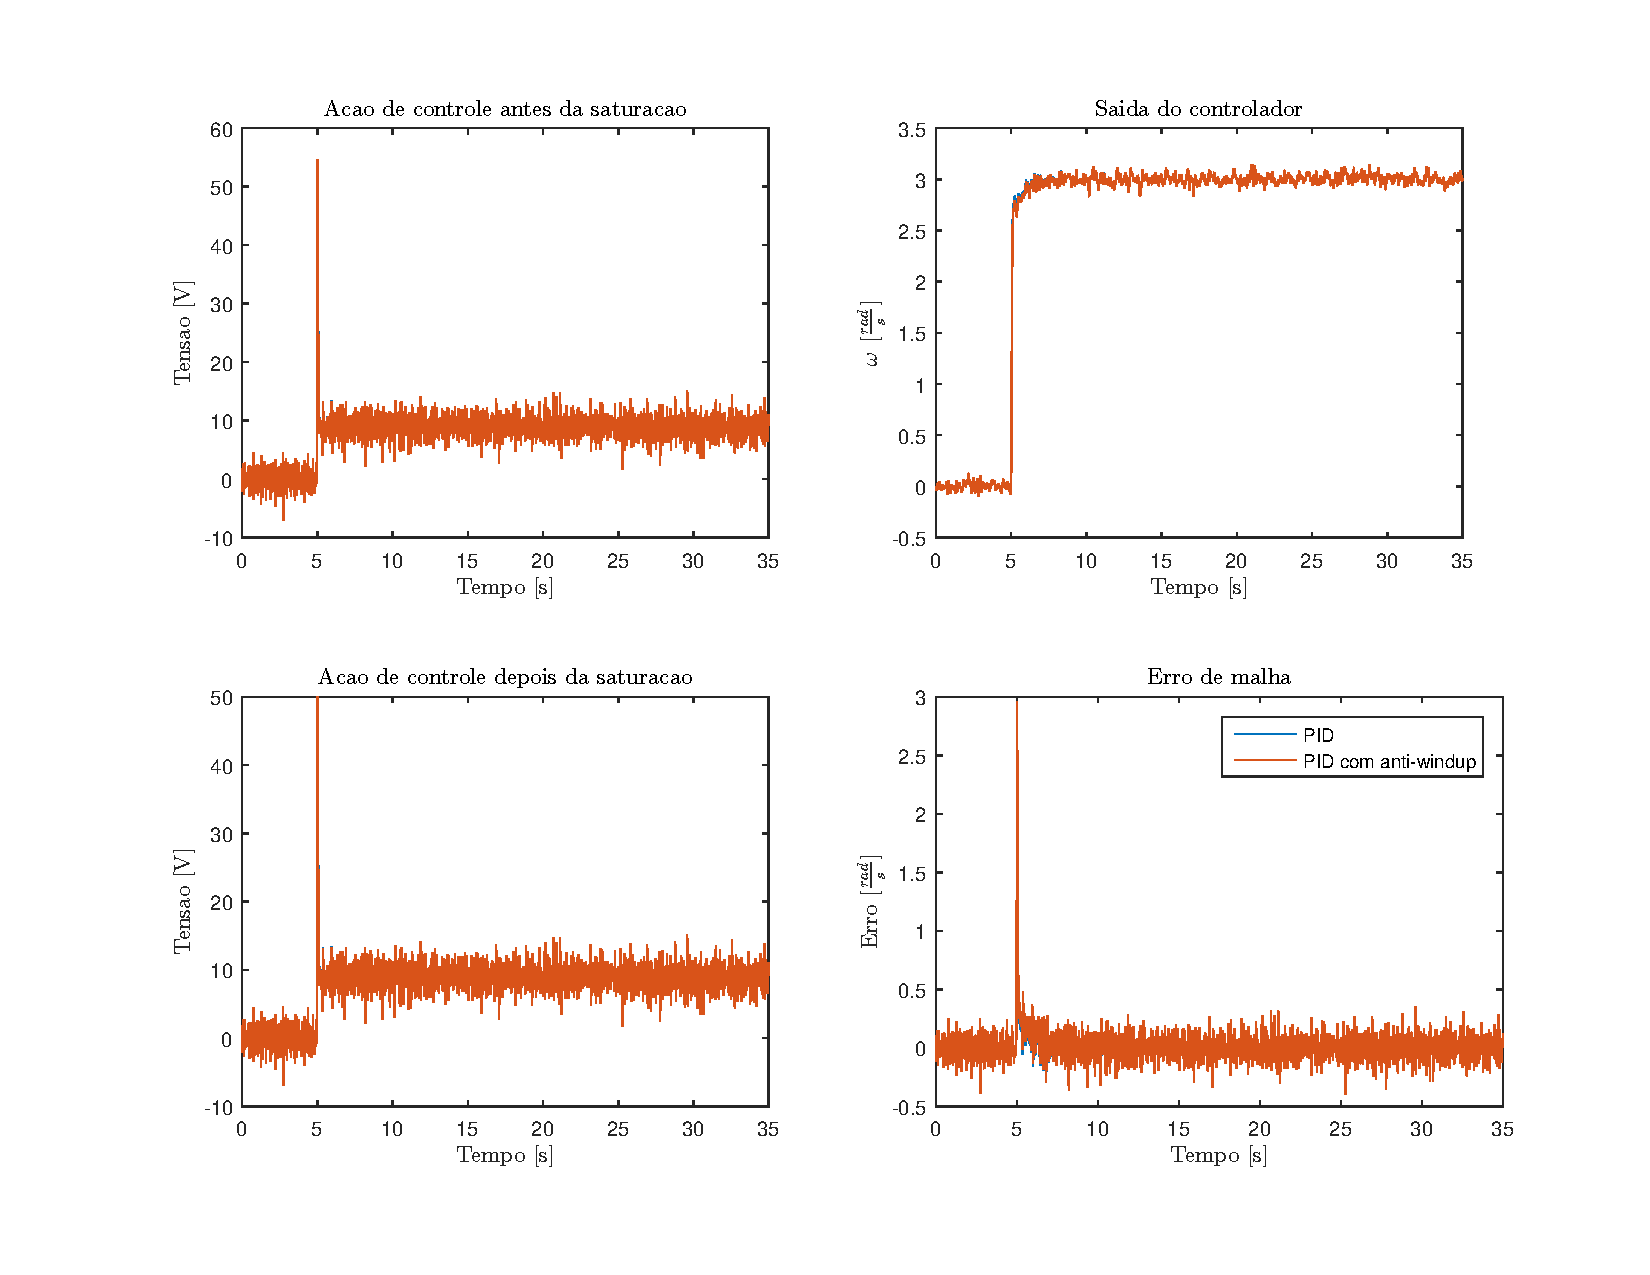
\includegraphics[width=0.7\textwidth, trim=3.5cm 2cm 2cm 1cm]{ex7PID_PIDantiwindup.pdf}
    \caption{Diagrama de blocos utilizado para exercício 7}
    \label{fig:PIDantiwindup}
\end{figure}

\begin{figure}[H]
    \center
    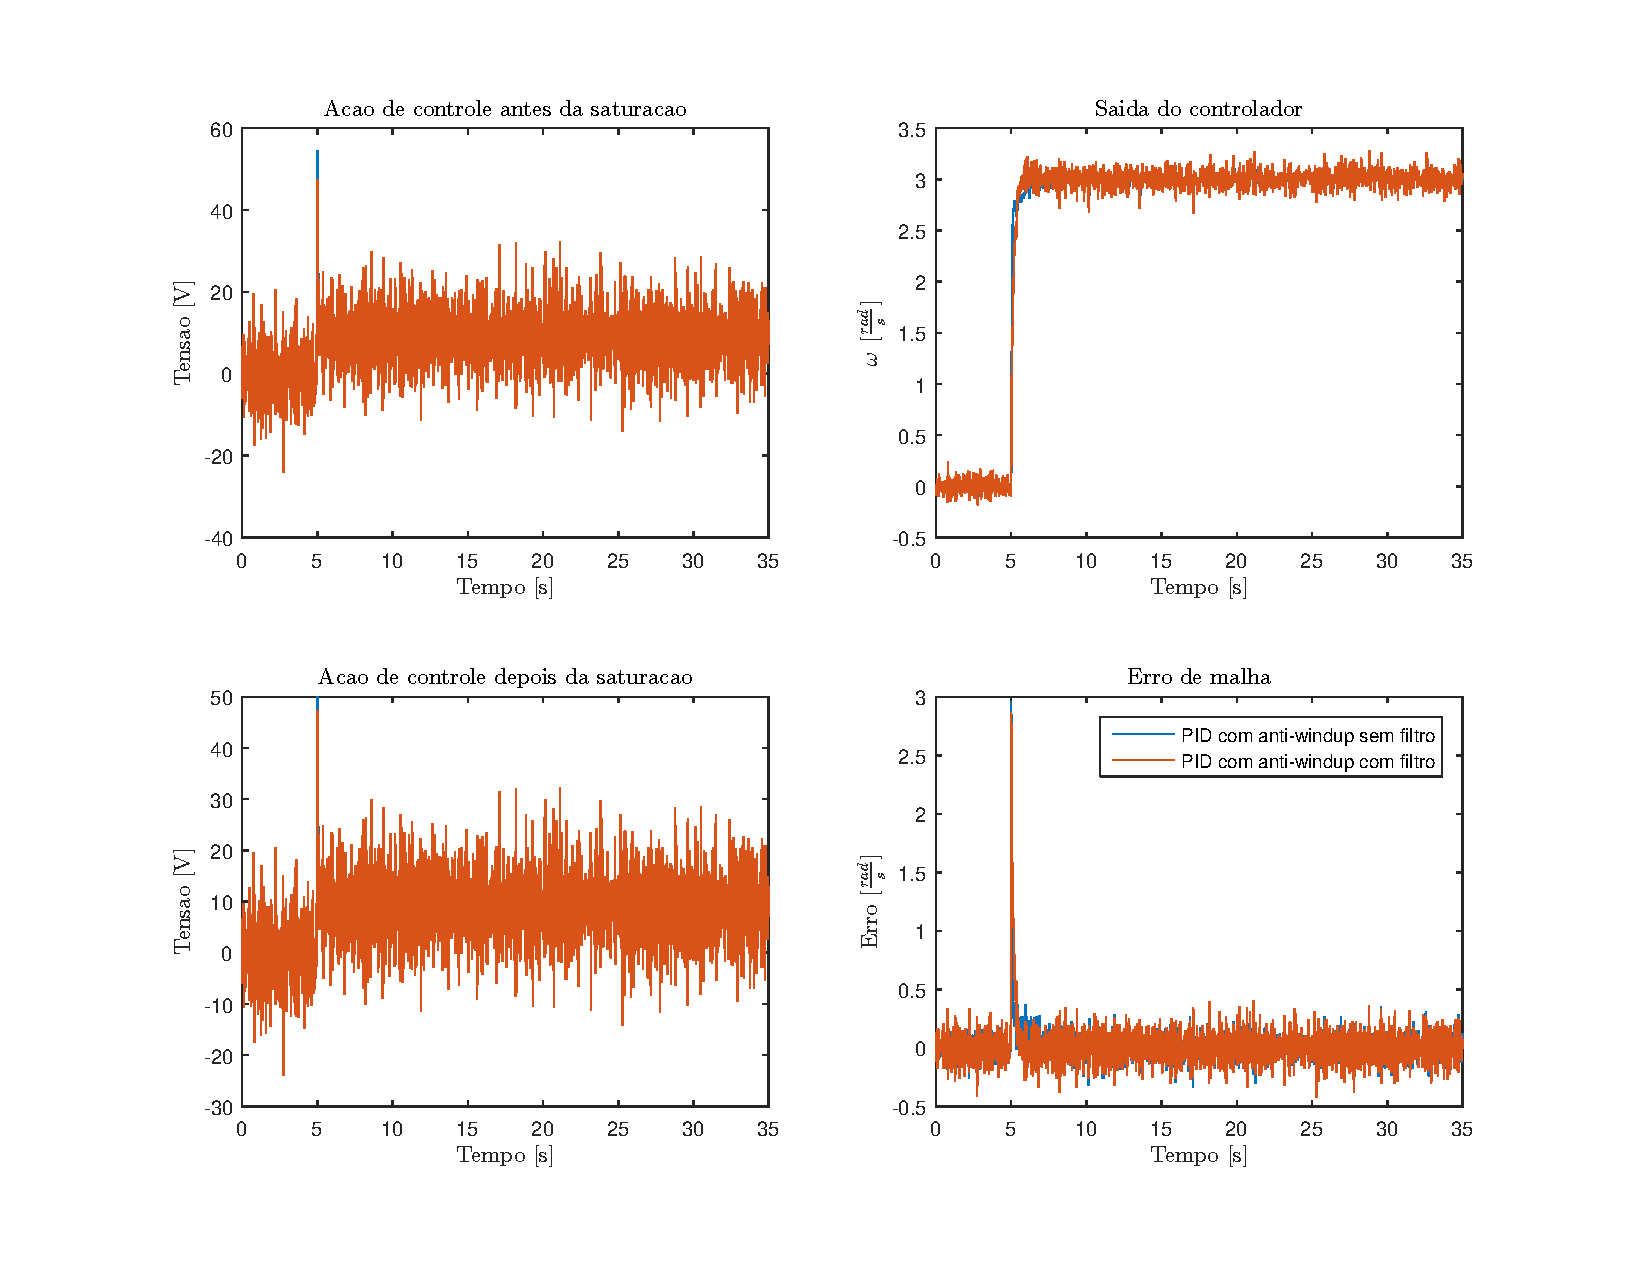
\includegraphics[width=0.8\textwidth, trim=3.5cm 2.5cm 2cm 2cm]{ex7PID_antiwindup_filtro.pdf}
    \caption{Diagrama de blocos utilizado para exercício 7}
    \label{fig:PIDfiltro}
\end{figure}

\begin{figure}[H]
    \center
    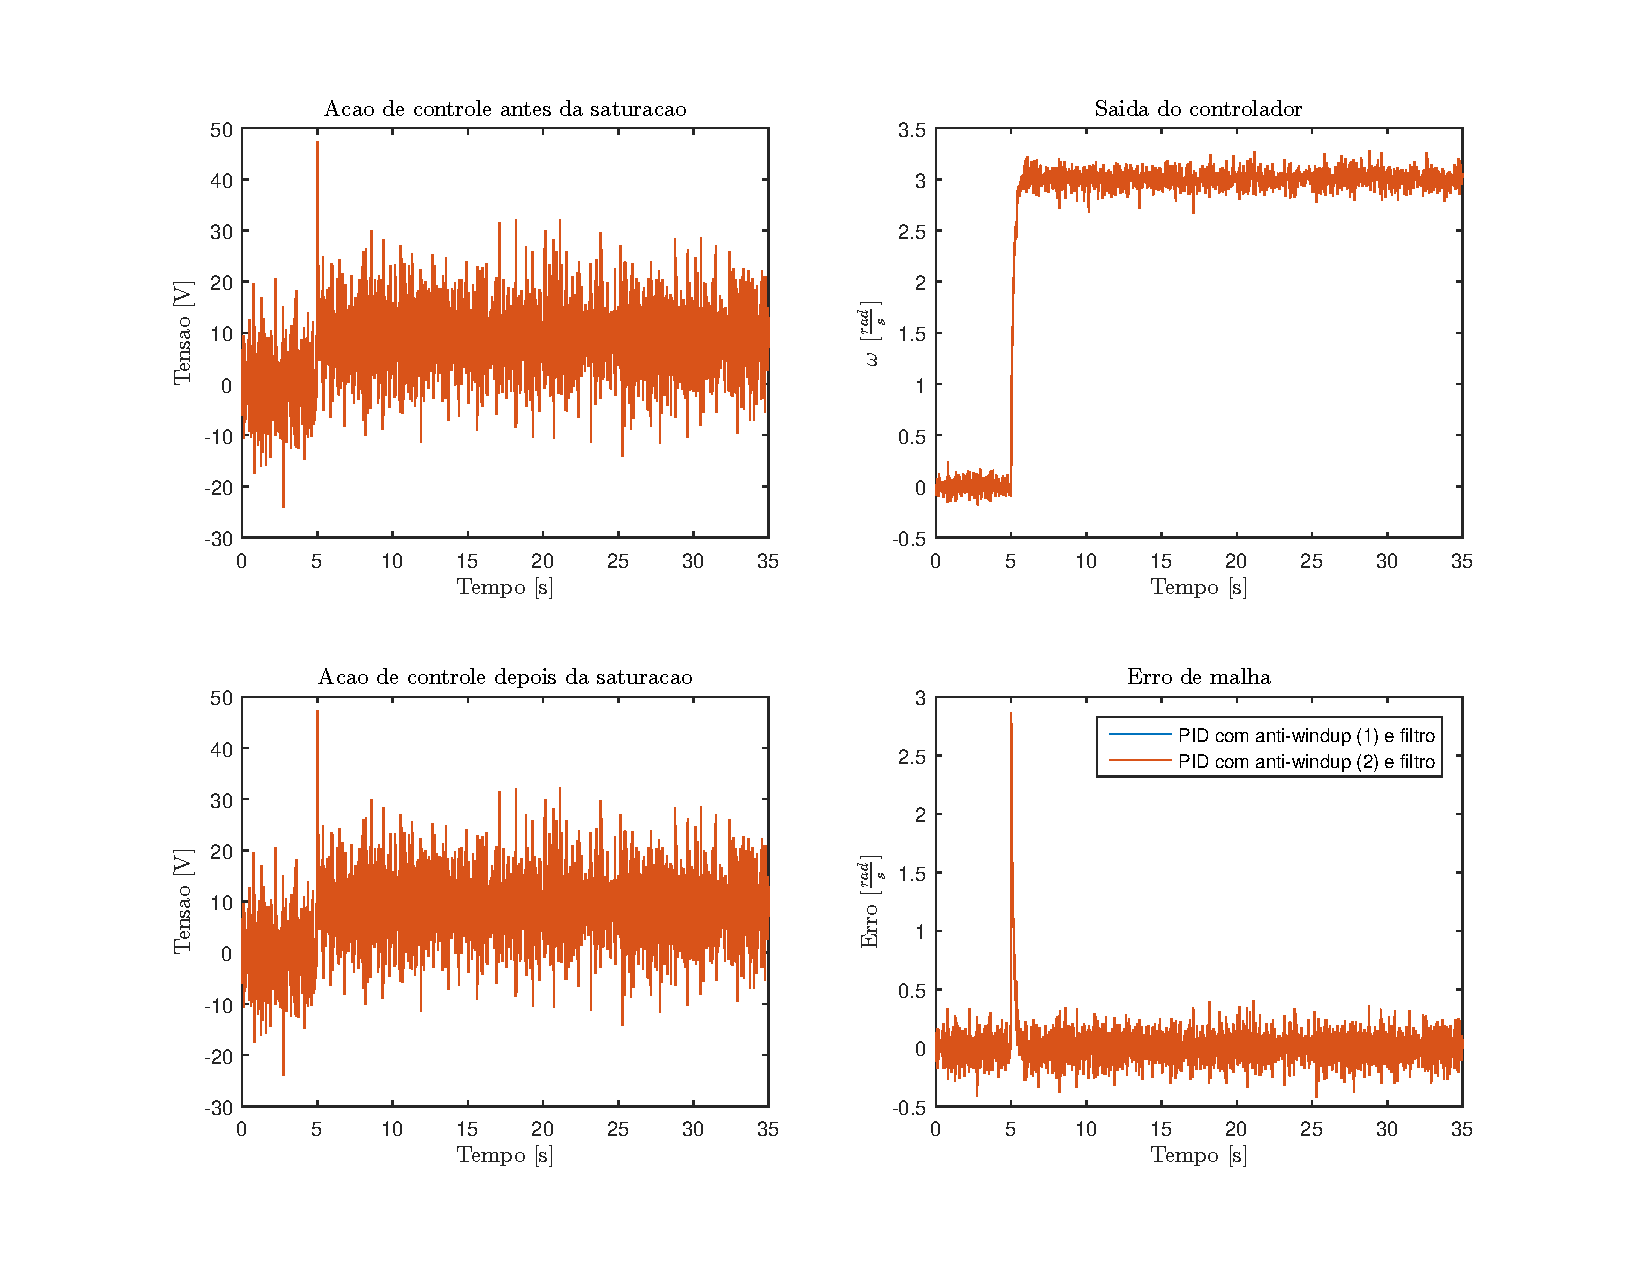
\includegraphics[width=0.8\textwidth, trim=3.5cm 2.5cm 2cm 2cm]{PID_antiwidup12_filtro.pdf}
    \caption{Diagrama de blocos utilizado para exercício 7}
    \label{fig:PIDantiwindup12}
\end{figure}

\begin{figure}[H]
    \center
    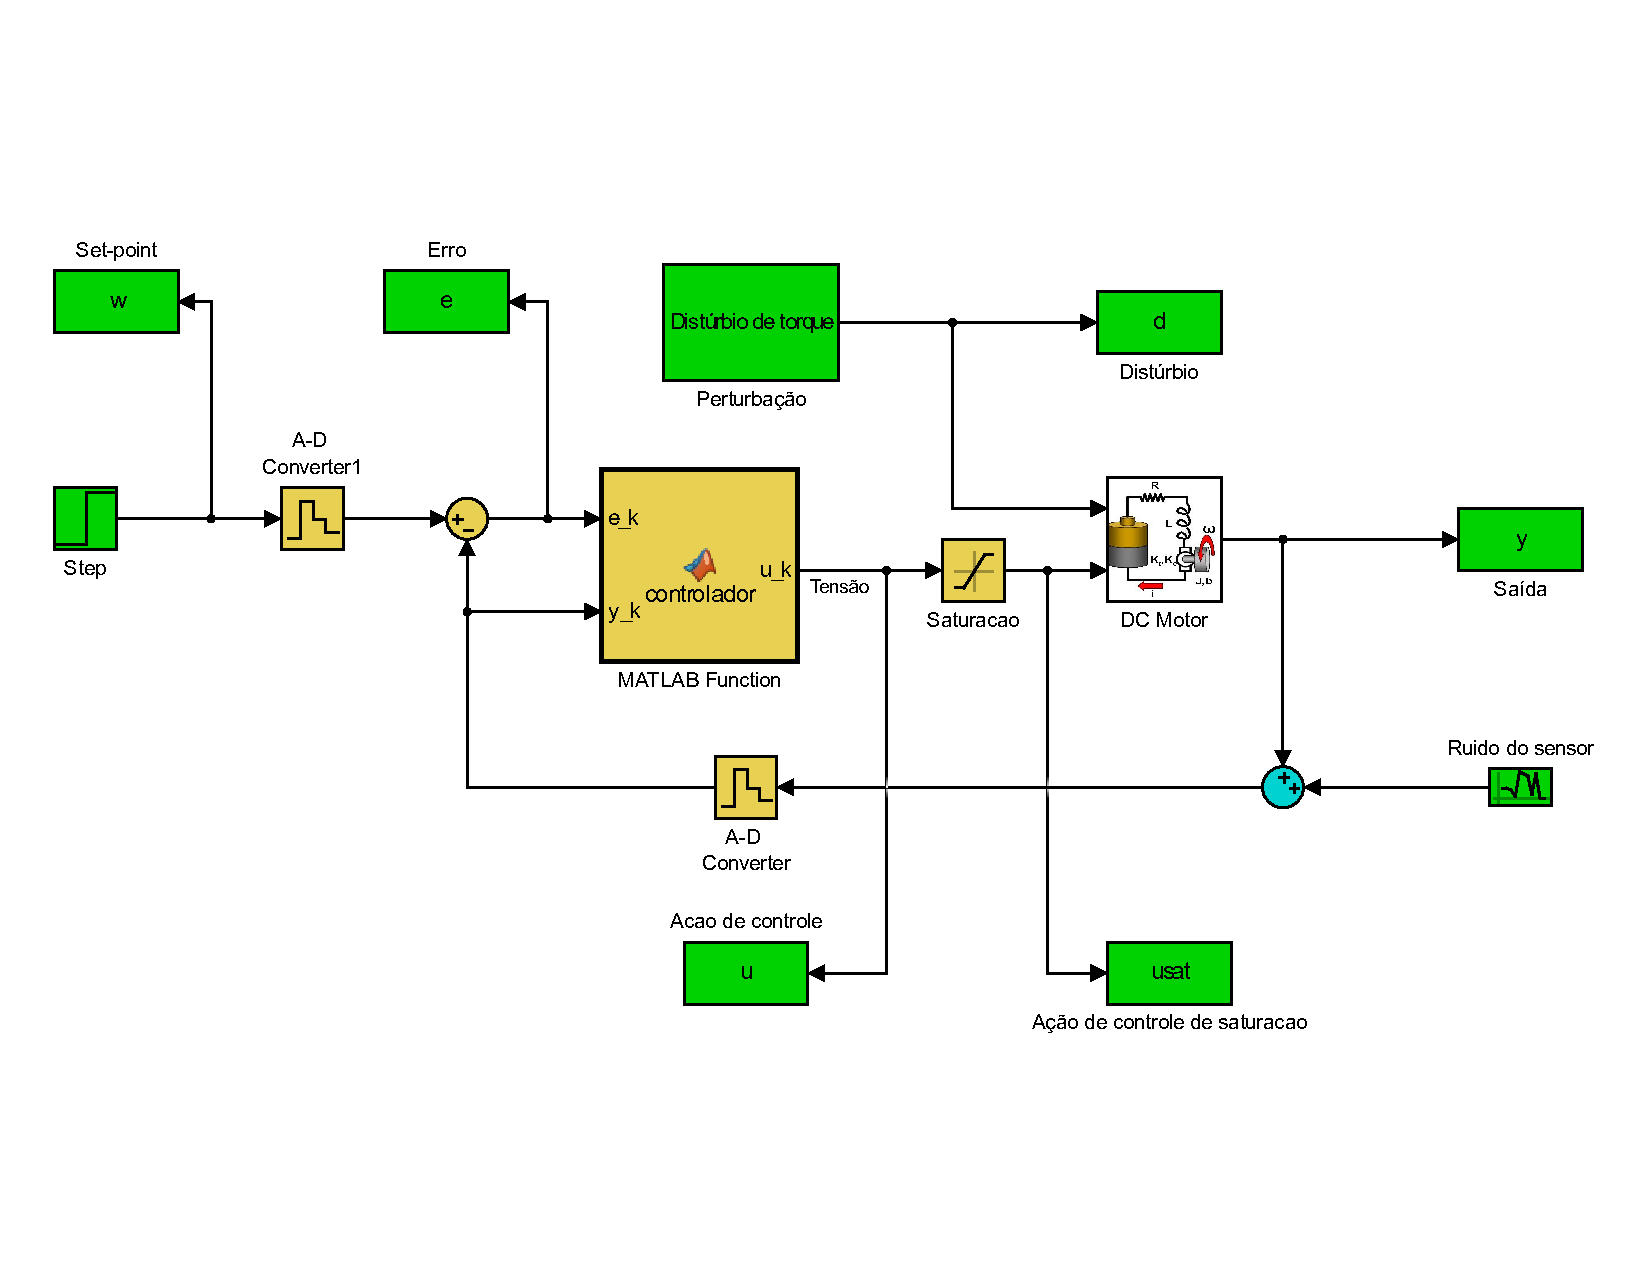
\includegraphics[width=0.7\textwidth, trim=4cm 3.5cm 1cm 2cm]{dcIntrocomplete.pdf}
    \caption{Principais sinais de controle do diagrama} 
    \label{fig:dcIntrocomplete}
\end{figure}